\section{Implementierung von Reglern}
\begin{multicols}{2}
Es wird eine minimale Implementierung angestrebt, was bedeutet, dass die Anzahl
der Integratoren minimal sein soll. Wenn der gegebene Regler $G_R(s)$ vollständig
gekürzt ist, dann hat eine minimale Implementierung n Integratoren.
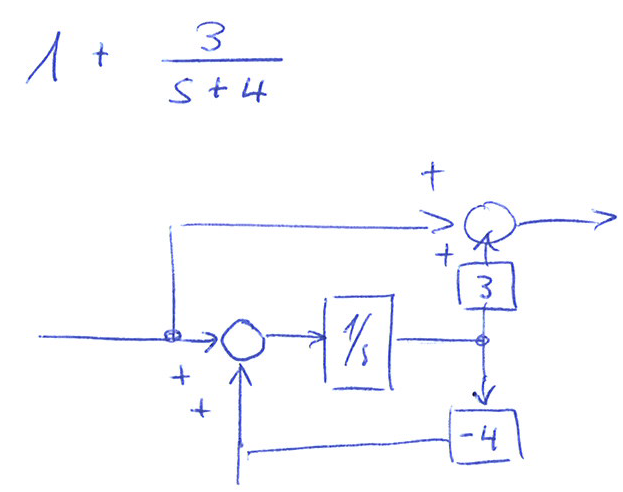
\includegraphics[width=5cm]{./images/implementierung2.png}
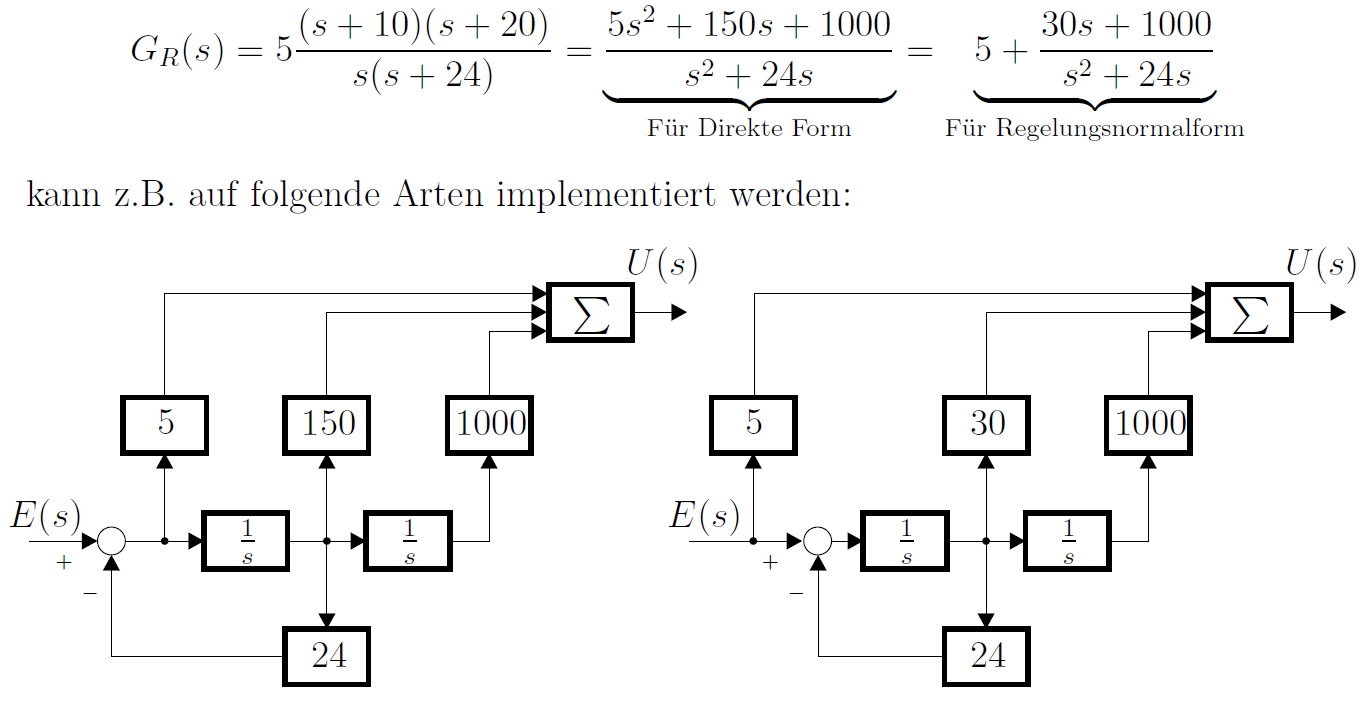
\includegraphics[width=10cm]{./images/implementierung.png}
\end{multicols}
